%\documentclass{article}
%\usepackage{graphicx,subfigure}
%\begin{document}

\begin{figure}[!h]
  \centering
  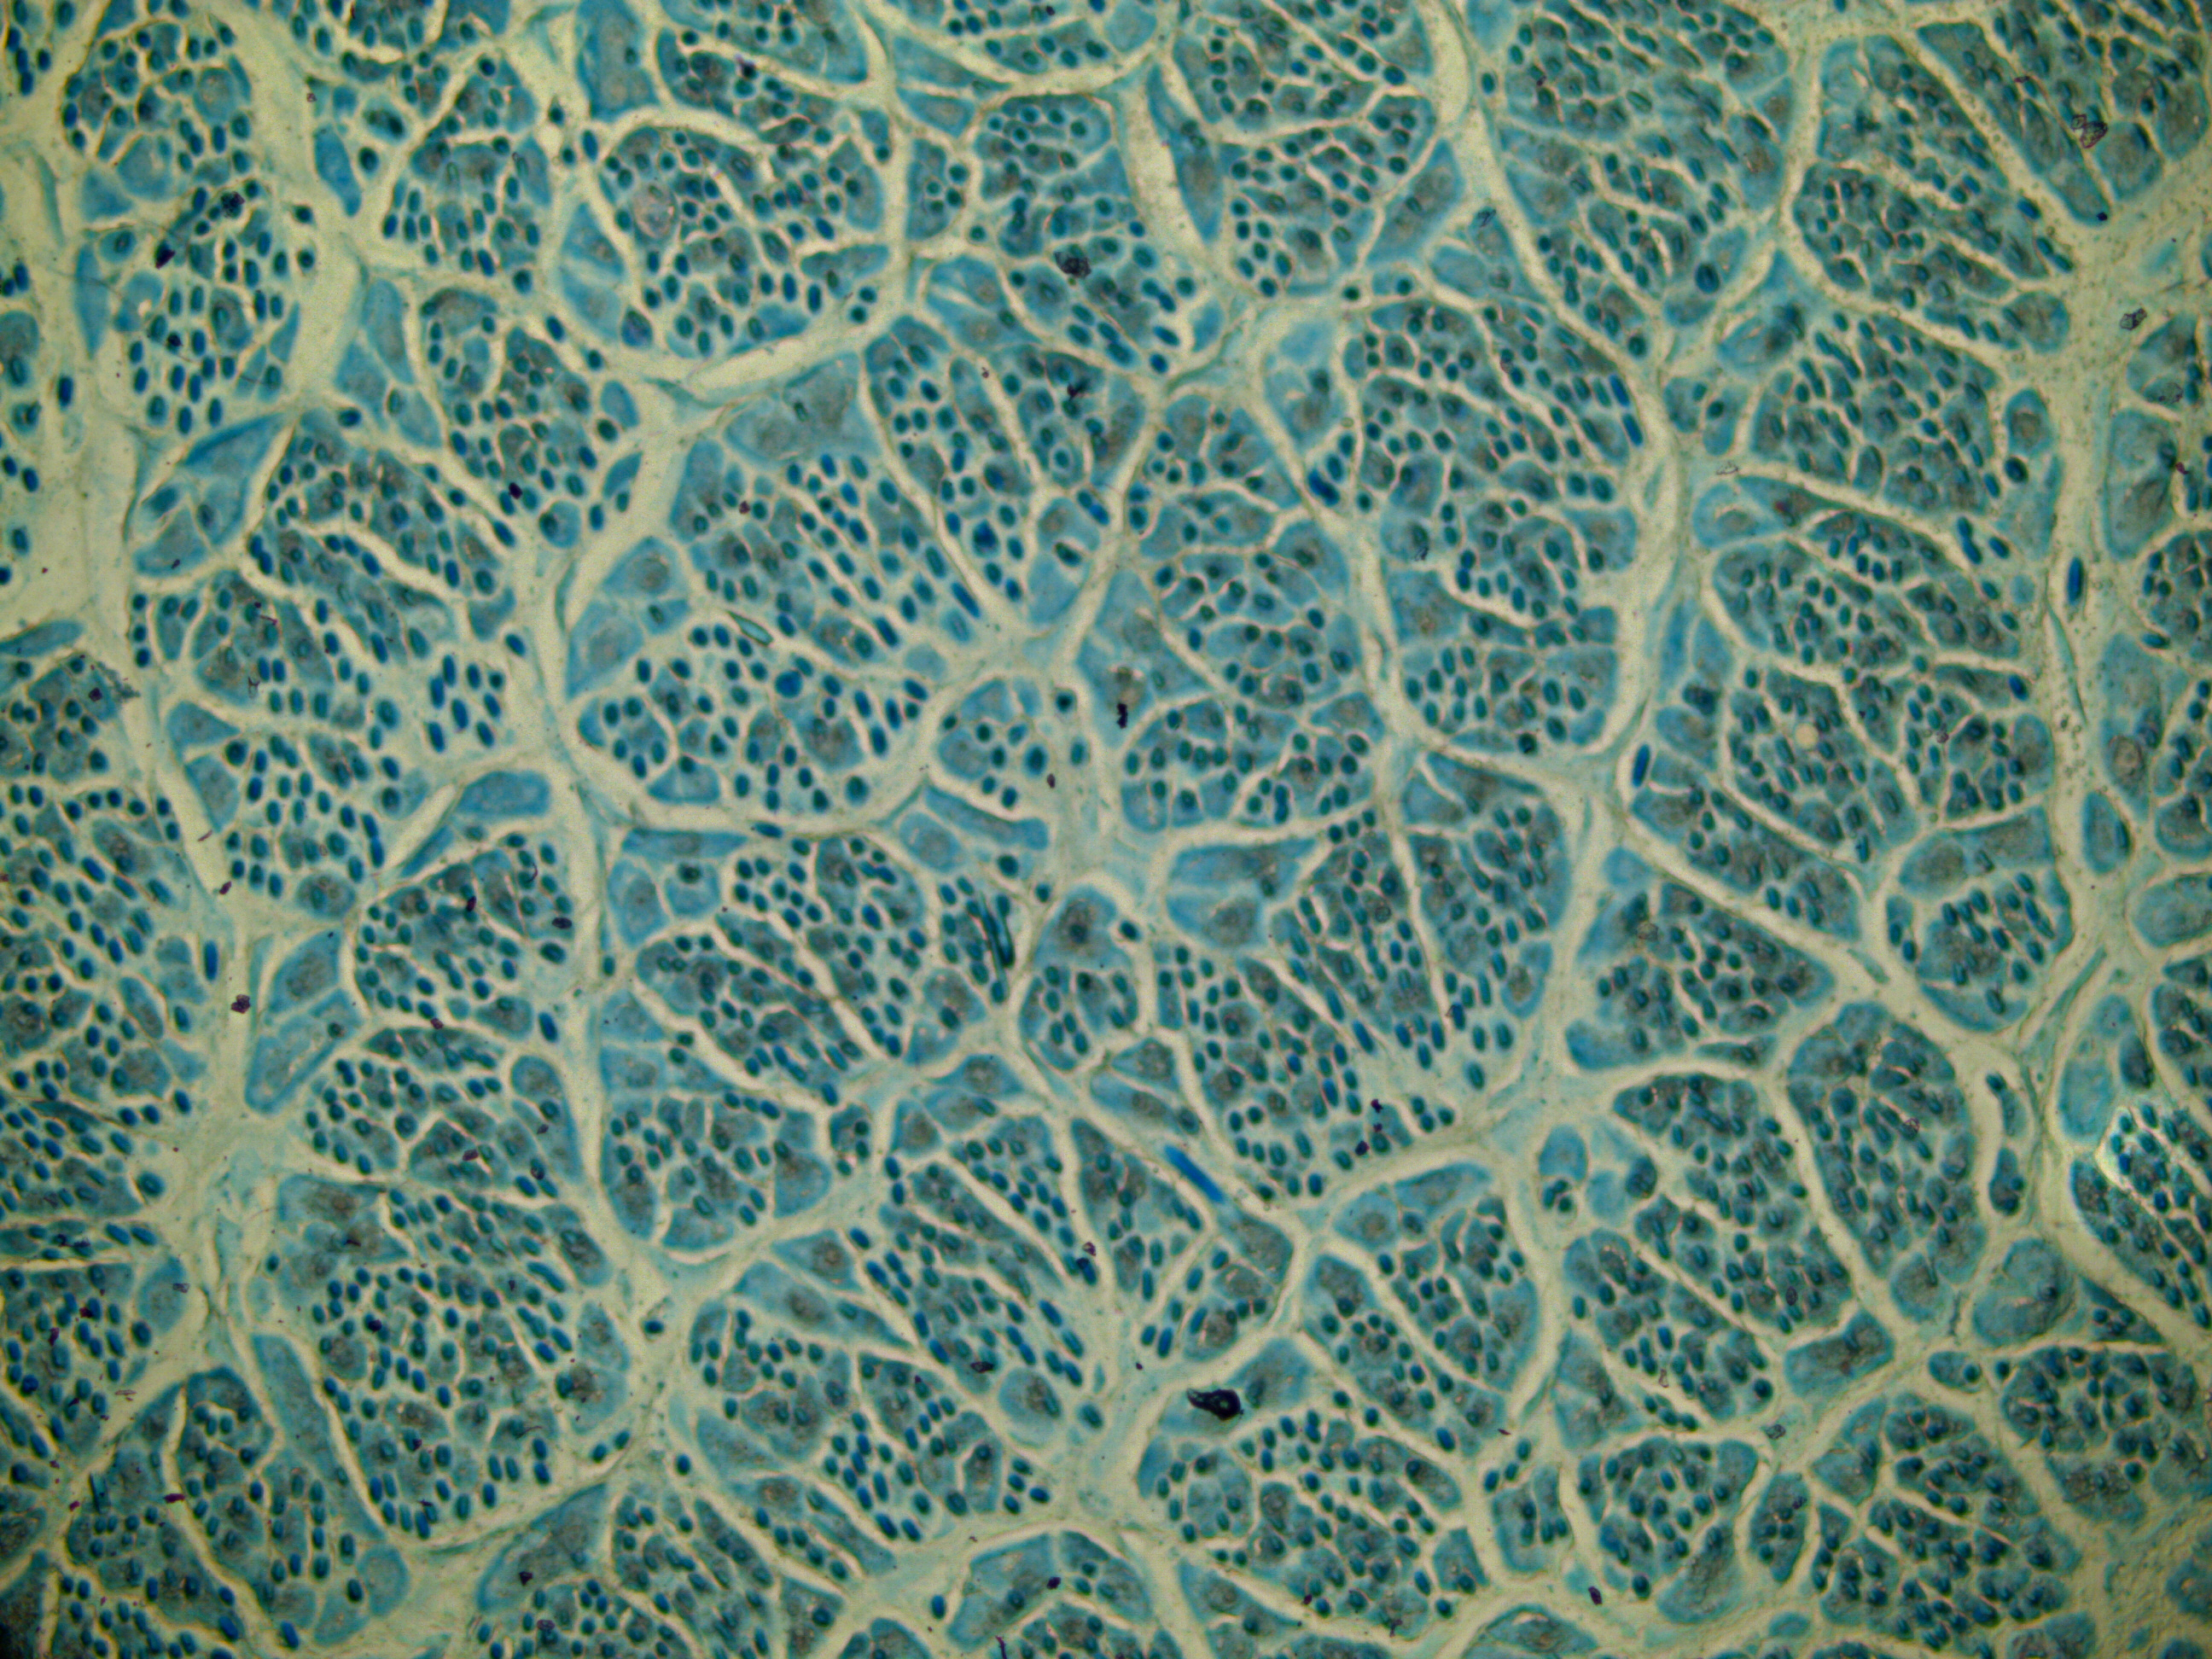
\includegraphics[width=1.0\textwidth,angle=90]{figskinhs.jpg}
% 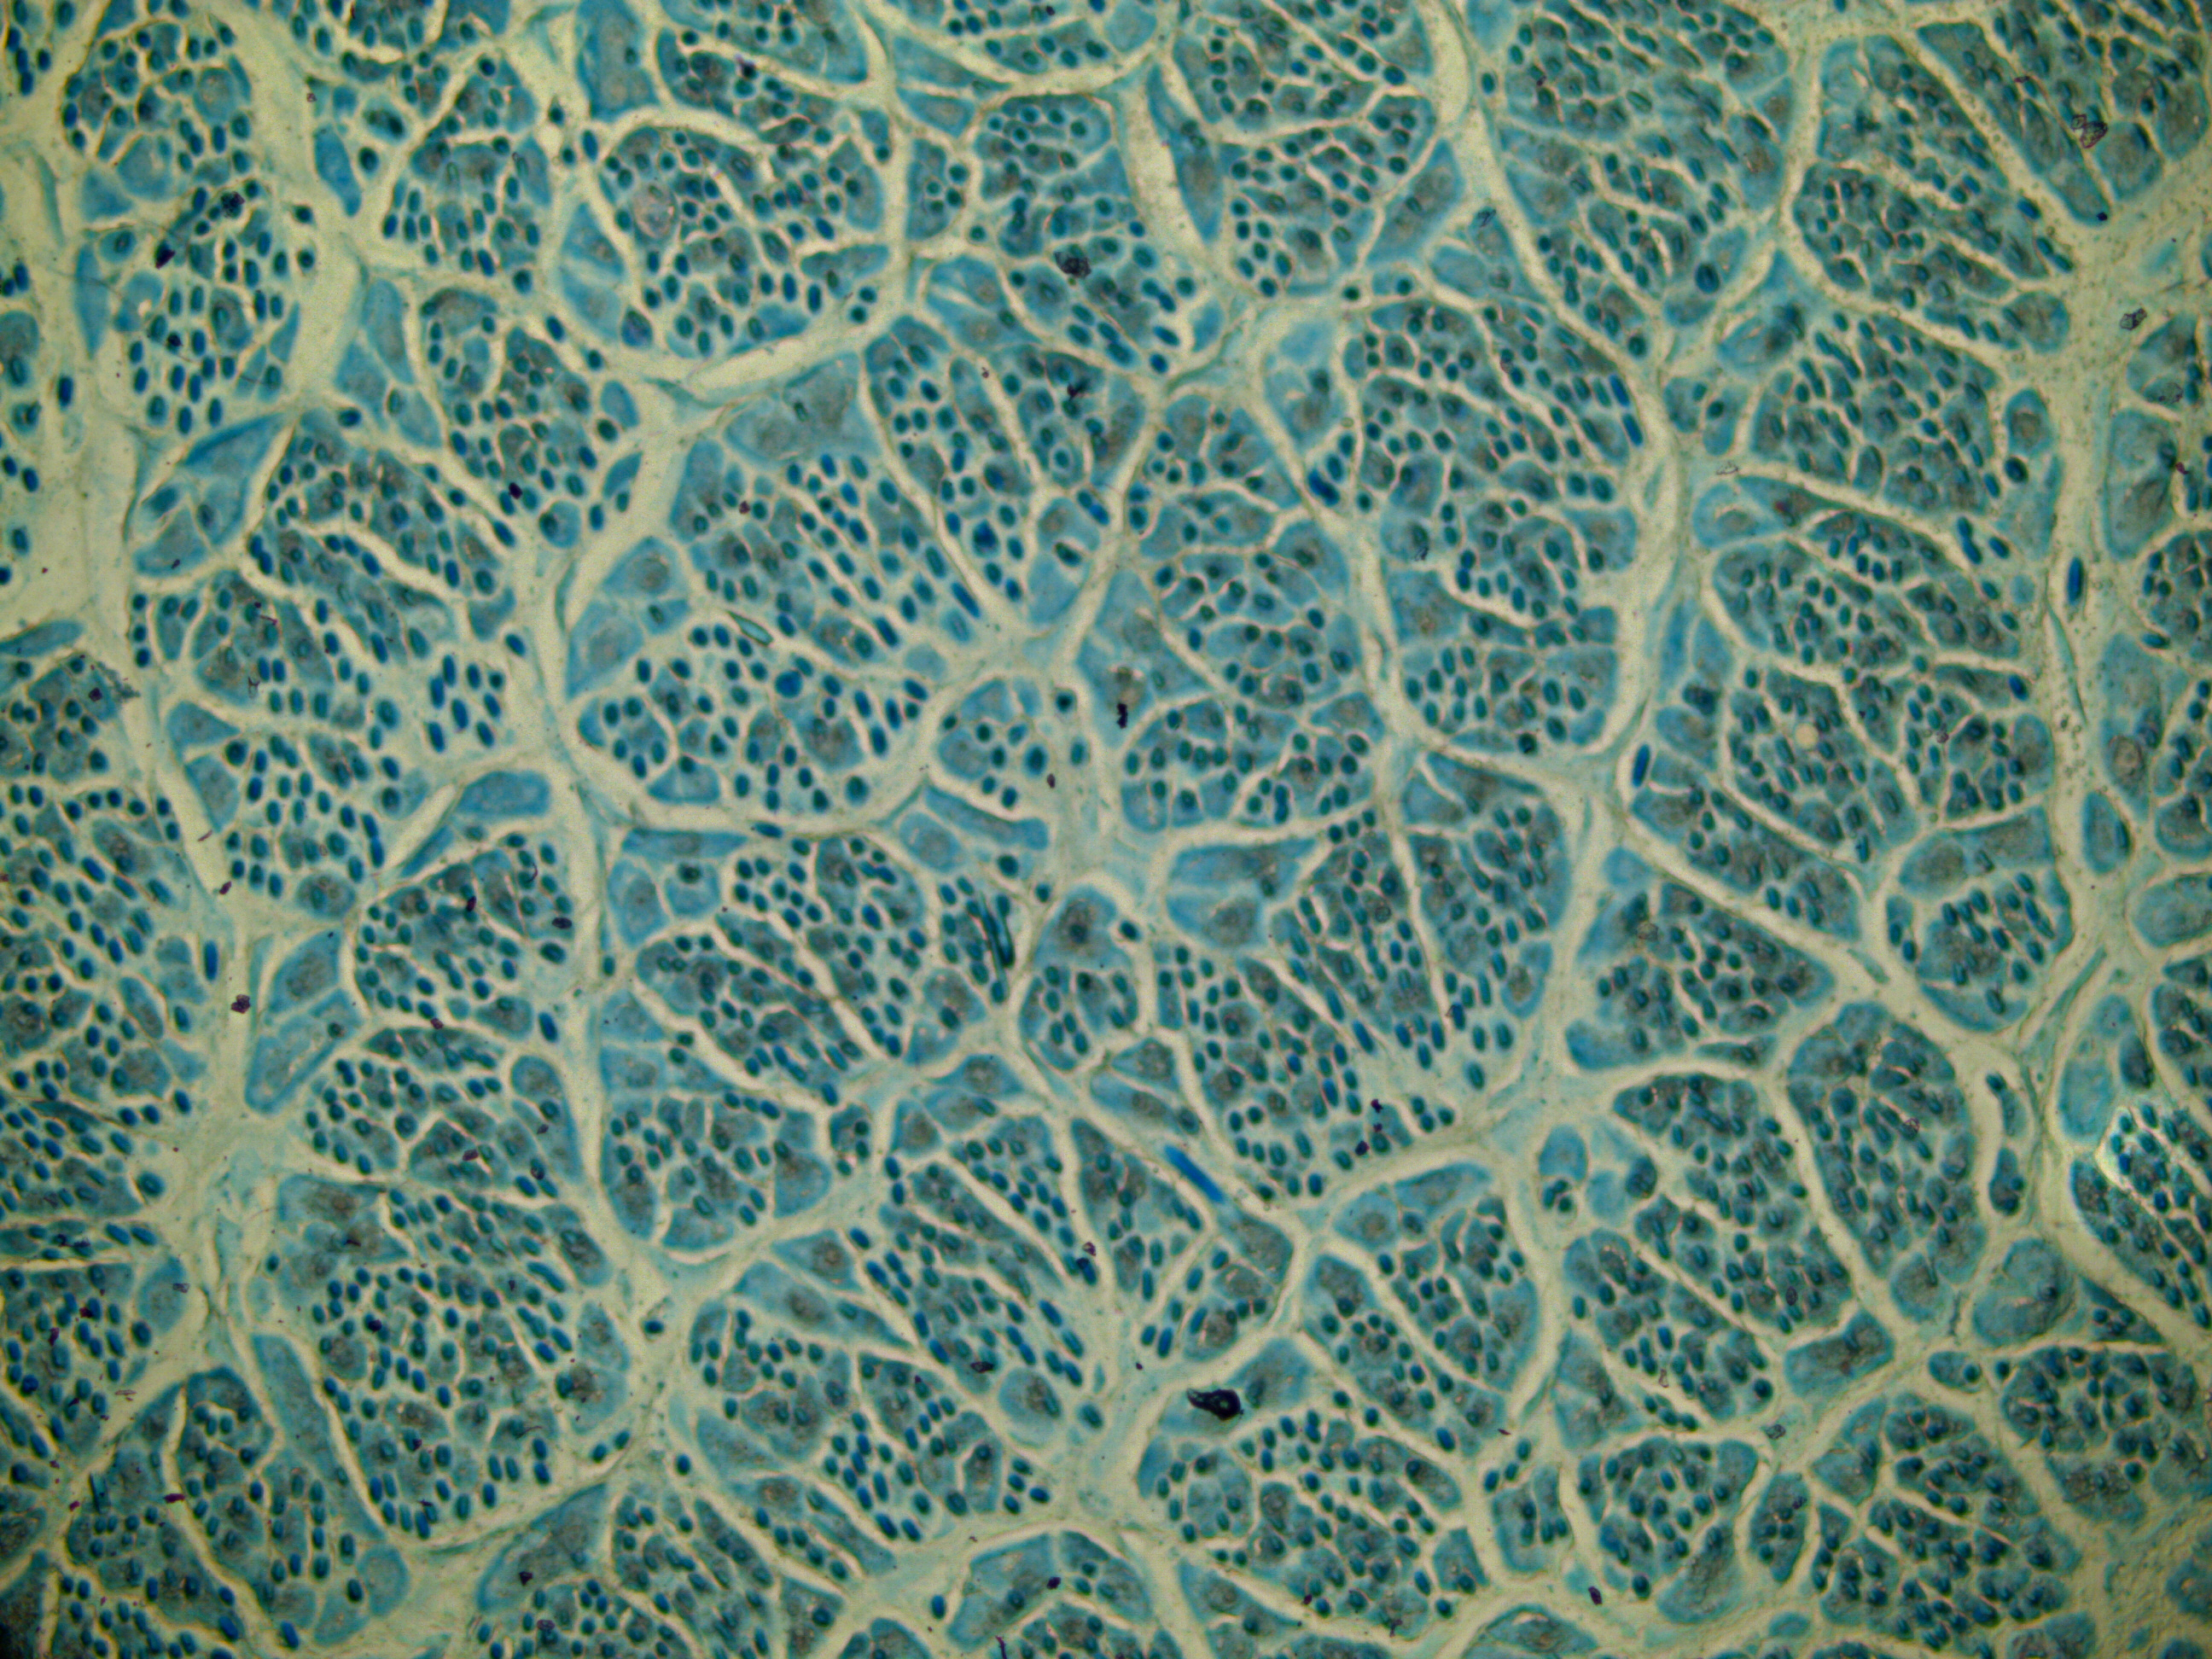
\includegraphics[width=1.0\textwidth]{figskinhs.jpg}
% 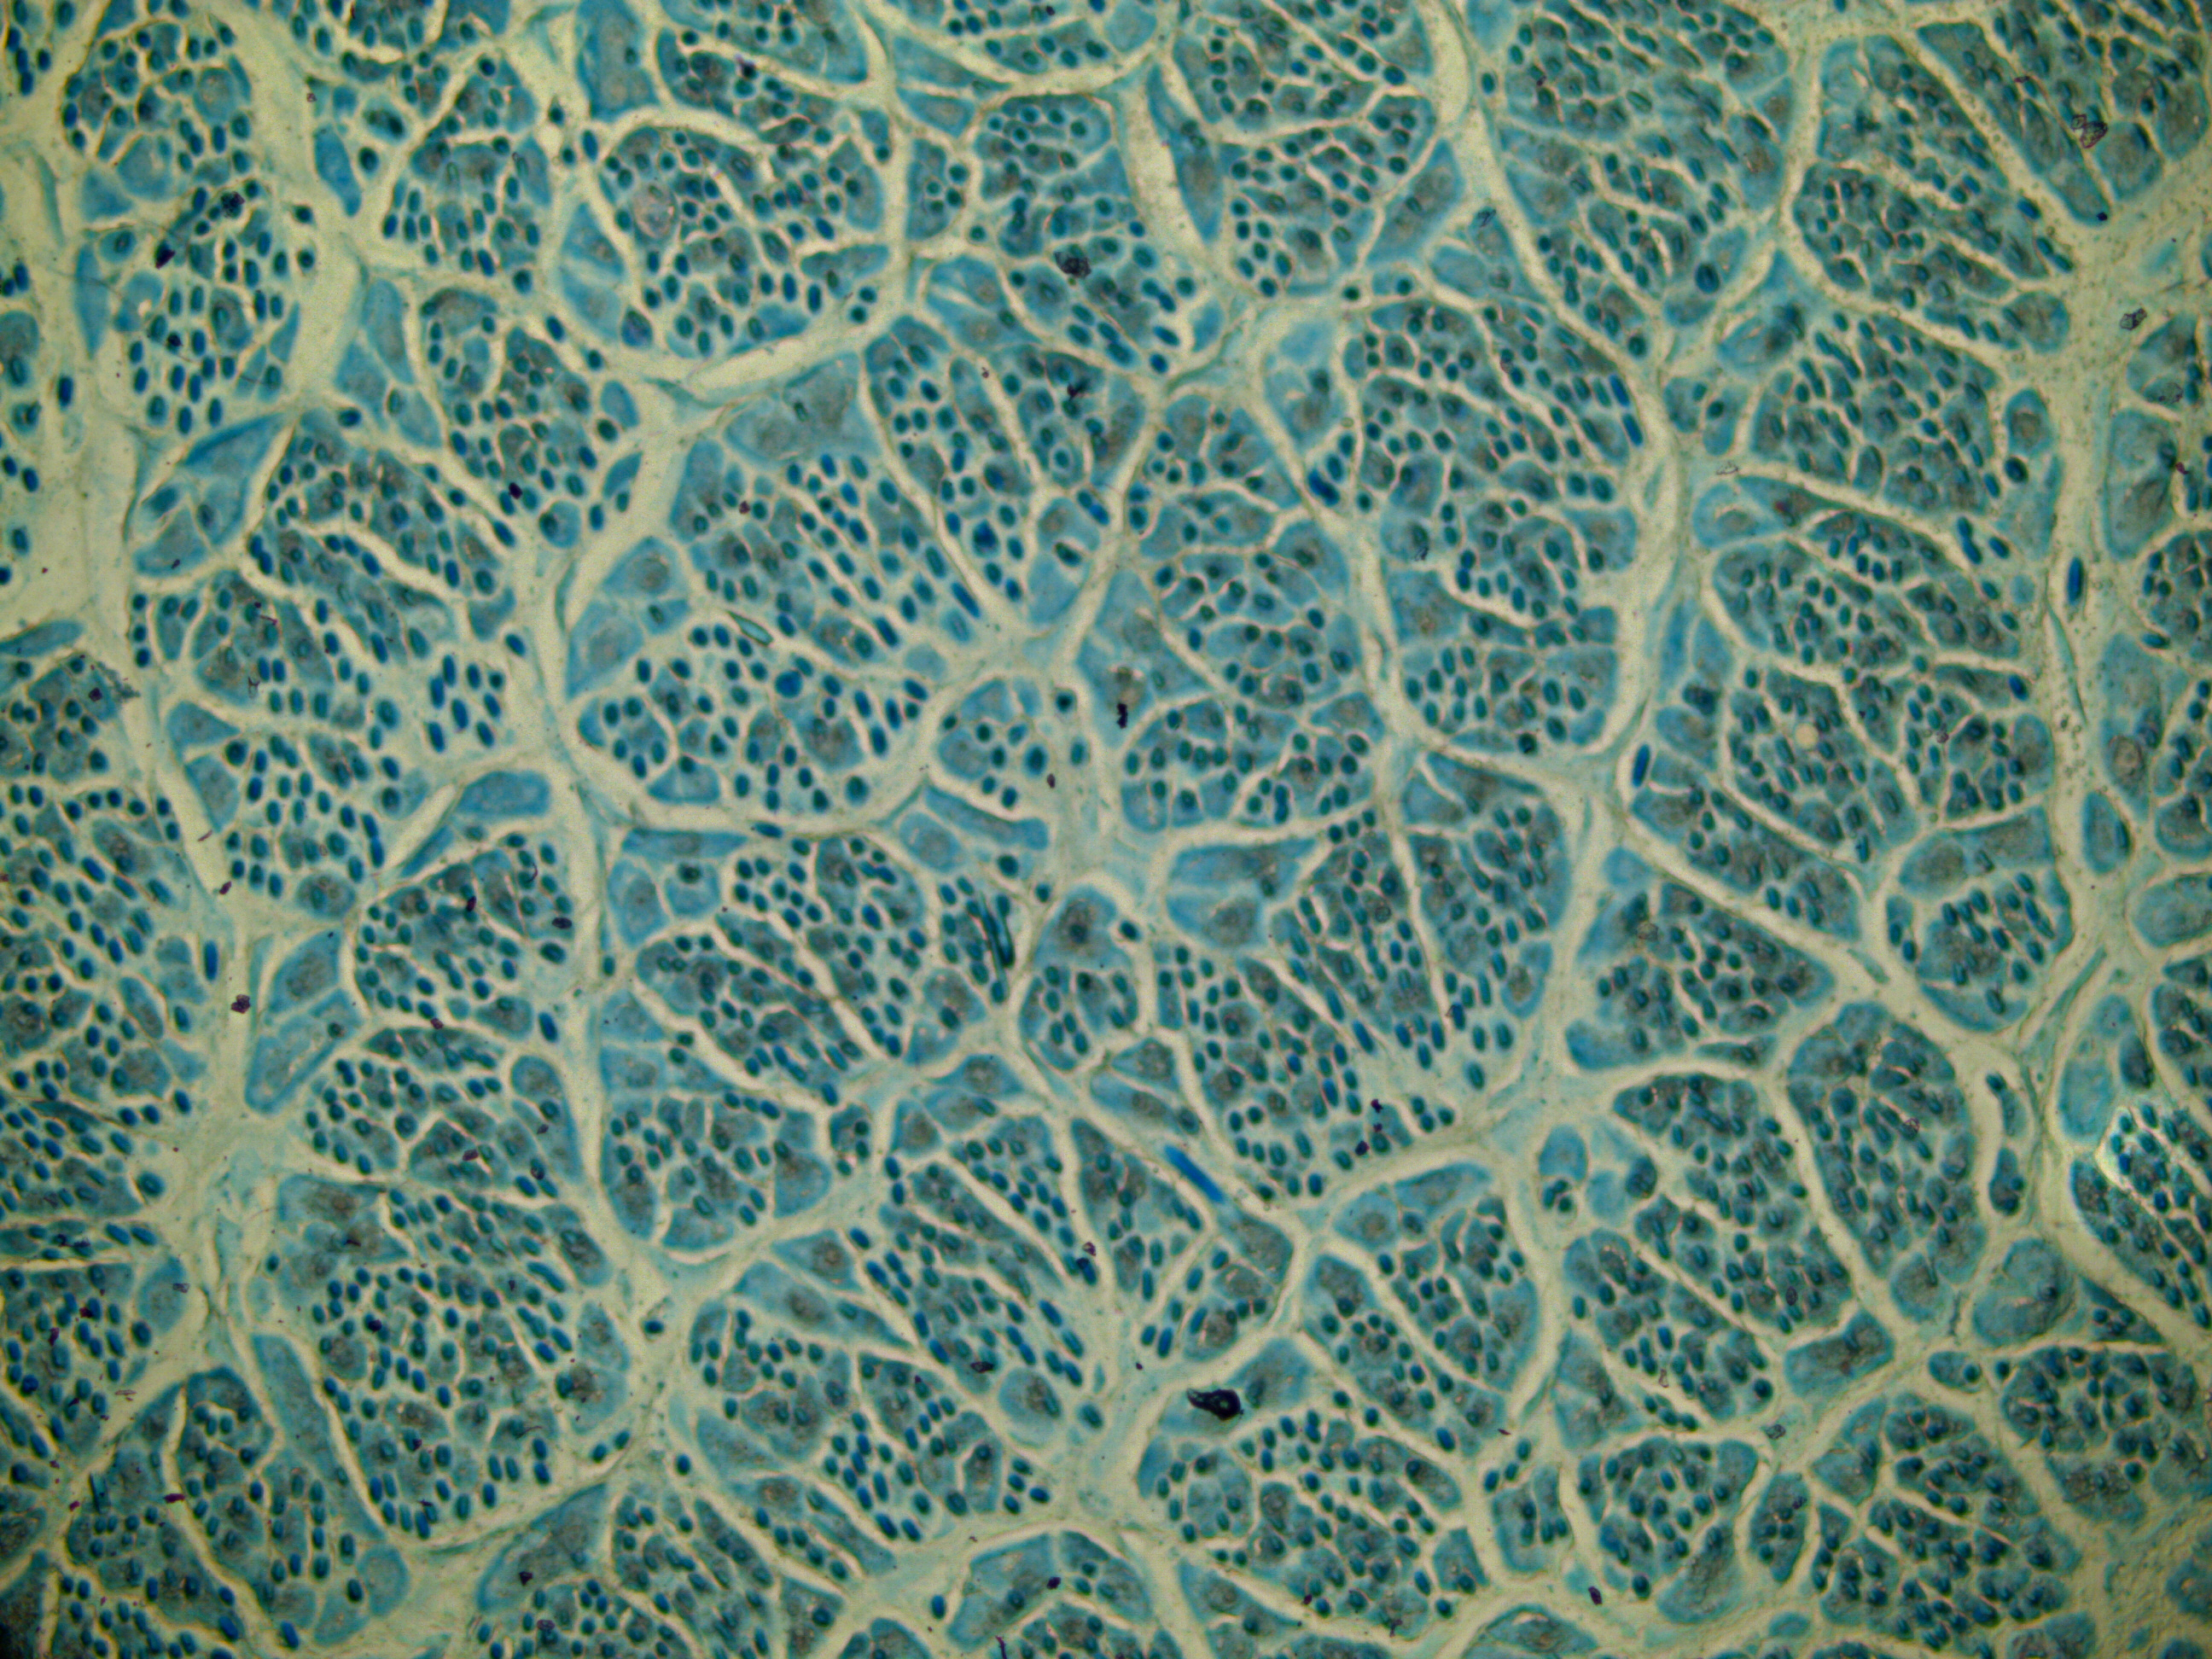
\includegraphics[scale=0.18]{figskinhs.jpg}
  \caption{A horizontal skin section from a Merino sheep with unfolded helix crimp showing rows of follicle groups with appreciable connective tissue space between the rows. The direction referred to as north-south is vertical and east-west is horizontal. 25x magnification. Stained with Nile Blue sulphate}
  \label{skin:hs}
\end{figure}

%\end{document}

